% -*- coding: utf-8 -*-

\documentclass[10pt,dvipdfmx]{beamer}
\usepackage{tutorial}
\title{計算機実験 --- 数値計算の基礎}

\begin{document}

\begin{frame}
  \titlepage
  \tableofcontents
\end{frame}

\section{数値誤差}

\begin{frame}[t,fragile]{数値誤差の原因}
  \begin{itemize}
    \setlength{\itemsep}{1em}
  \item 丸め誤差: 無理数や10進数を有限のビットの2進数で表現することによる誤差
    (例: 0.1 が 0.0999999999998 になる)
  \item 打ち切り誤差: テイラー展開による近似を有限項で打ち切ることによる誤差
    (例: 数値微分)
  \item 桁落ち: 非常に近い数の引き算により生じる
  \item 情報落ち: 非常に大きな数に小さな数を足し込む場合に生じる
    (例: 数値積分や常微分方程式の初期値問題で刻み幅を小さくしすぎると生じる)
  \item オーバーフロー(桁あふれ): 表現できる値を超えてしまう
  \end{itemize}
\end{frame}

\begin{frame}[t,fragile]{桁落ち}
  \begin{itemize}
    \setlength{\itemsep}{1em}
  \item 2次方程式 $ax^2+bx+c=0$の解の公式
    \[
    x_{\pm} = \frac{-b \pm \sqrt{b^2-4ac}}{2a}
    \]
    $b^2 \gg |ac|$の時、桁落ちが生じる
  \item 例) $2.718282x^2 - 684.4566x+0.3161592=0$ の解を7桁の精度で計算してみる(伊理・藤野1985)
    \begin{align*}
      \sqrt{D} &= \sqrt{(684.4566)^2 - 4 \times 2.718282 \times 0.3161592} = 684.4541 \\
      x_+ &= \frac{684.4566+684.4541}{2 \times 2.718282} = \frac{1368.911}{5.436564} = 251.7970 \\
      x_- &= \frac{684.4566-684.4541}{2 \times 2.718282} = \frac{0.0025}{5.436564} = 0.00045\underline{98493}
    \end{align*}
  \end{itemize}
\end{frame}

\begin{frame}[t,fragile]{桁落ちを防ぐ方法}
  \begin{itemize}
    \setlength{\itemsep}{1em}
  \item $b$の符号に応じて、一方を求める(この例では$x_+$)
  \item 他方は解と係数の関係を使って求める
    \[
    x_- = \frac{c/a}{x_+} = \frac{0.3161592 / 2.718282}{251.7970} = 0.000461913\underline{8}
    \]
  \item 回避できない例: 重解に近い場合 $2.718282x^2 - 1.854089x + 0.3161592=0$
    \begin{align*}
      \sqrt{D} &= \sqrt{(1.854089)^2 - 4 \times 2.718282 \times 0.3161592} \\ &= 0.002\underline{64575} \\
      x_\pm &= 1.854089 \pm 0.002\underline{64575} = 1.856\underline{737}, 1.851\underline{445}
    \end{align*}
  \end{itemize}
\end{frame}

\begin{frame}[t,fragile]{数値微分}
  \begin{itemize}
    \setlength{\itemsep}{1em}
  \item 関数のテイラー展開
    \[
    f(x+h) = f(x) + h f'(x) + h^2 f''(x)/2 + h^3 f'''(x)/6 + \cdots
    \]
  \item 数値微分の最低次近似
    \[
    f_1(x,h) \equiv \frac{f(x+h)-f(x)}{h} = f'(x) + h f''(x)/2 + O(h^2)
    \]
  \item より高次の近似
    \[
    f_2(x,h) \equiv \frac{f(x+h)-f(x-h)}{2h} = f'(x) + h^2 f'''(x)/6 + O(h^3)
    \]
  \item 刻み$h$を小さくすると打ち切り誤差は減少するが、小さすぎると今度は桁落ちが大きくなる
  \end{itemize}
\end{frame}

\begin{frame}[t,fragile]{刻み幅を変えた計算}
  \begin{itemize}
    \setlength{\itemsep}{1em}
  \item 刻み幅を変えて何度か計算を行い、収束の様子をみる
  \item グラフ化して目で見てみる
  \item 理論式と比較
    \begin{itemize}
    \item 計算式の正しさの確認
    \item 近似の改良 (収束の加速・補外)
    \end{itemize}
  \item 桁落ち・情報落ちの影響の有無
  \end{itemize}
\end{frame}

% -*- coding: utf-8 -*-

\section{ニュートン法}

\begin{frame}[t,fragile]{ニュートン法}
  \begin{itemize}
    \setlength{\itemsep}{1em}
  \item 反復法により方程式$f(x)=0$の解を求める
  \item 真の解を$x_0$、現在の解の候補を$x_n=x_0+\epsilon$とすると
    \[
    0 = f(x_0) = f(x_0+\epsilon-\epsilon) = f(x_n) - f'(x_n) \epsilon + O(\epsilon^2)
    \]
  \item 次の解の候補 (反復法、逐次近似法)
    \[
    \epsilon \approx \frac{f(x_n)}{f'(x_n)} \quad\quad x_{n+1} = x_n - \frac{f(x_n)}{f'(x_n)}
    \]
  \item 複素変数の複素関数や多変数の場合にも自然に拡張可
  \end{itemize}
\end{frame}

\begin{frame}[t,fragile]{ニュートン法の収束}
  \begin{itemize}
    \setlength{\itemsep}{1em}
  \item $x_n$が$x_0$に十分近い時
    \begin{align*}
      f(x_n) &\approx f'(x_0) (x_n-x_0) + f''(x_0) \frac{(x_n - x_0)^2}{2} \\
      f'(x_n) &\approx f'(x_0) + f''(x_0) (x_n - x_0)
    \end{align*}
  \item ニュートン法で一回反復すると
    \begin{align*}
      x_{n+1} =  x_n - \frac{f(x_n)}{f'(x_n)} &\approx x_n - (1-\frac{f''(x_0)}{f'(x_0)}\frac{(x_n-x_0)}{2})(x_n-x_0) \\
      (x_{n+1}-x_0) &\approx \frac{f''(x_0)}{2f'(x_0)} (x_n - x_0)^2
    \end{align*}
    \item 一回の反復で誤差が2乗で減る(正しい桁数が倍に増える) ⇒ 二次収束
  \end{itemize}
\end{frame}

\begin{frame}[t,fragile]{多次元の場合}
  \begin{itemize}
    \setlength{\itemsep}{1em}
  \item $f(x)=0$: $d$次元(非線形)連立方程式
  \item $x$は$d$次元のベクトル: $x = (x_1,x_2,\cdots,x_d)$
  \item $f(x)$も$d$次元のベクトル: $f(x) = (f_1(x), f_2(x),\cdots,f_d(x))$
  \item 真の解のまわりでの展開 ($x_n = x_0 + \epsilon$)
    \[
    0 = f(x_0) = f(x_0+\epsilon-\epsilon) = f(x_n) - \frac{\partial f(x_n)}{\partial x} \cdot \epsilon + O(|\epsilon|^2)
    \]
  \item ヤコビ行列($d\times d$): $\displaystyle \Big(\frac{\partial f(x_n)}{\partial x}\Big)_{ij} = \frac{\partial f_i(x_n)}{\partial x_j}$
  \item 次の解の候補: $\displaystyle x_{n+1} = x_n - \Big(\frac{\partial f(x_n)}{\partial x}\Big)^{-1} f(x_n)$
  \end{itemize}
\end{frame}

\begin{frame}[t,fragile]{ニュートン法による最適化}
  \begin{itemize}
    \setlength{\itemsep}{1em}
  \item $x$は$d$次元のベクトル: $x = {}^t(x_1,x_2,\cdots,x_d)$, $g(x)$はスカラー
  \item 勾配ベクトル: $\displaystyle [\nabla g(x)]_i = \frac{\partial g(x)}{\partial x_i}$
  \item 極小値(最小値)となる条件: $\nabla g(x)=0$
  \item ニュートン法で$f(x)$を$\nabla g(x)$で置き換えればよい
  \item 次の解の候補: $\displaystyle x_{n+1} = x_n - H^{-1}(x_n) \nabla g(x_n)$
  \item ヘッセ行列(Hessian): $\displaystyle H_{ij}(x_n) = \frac{\partial^2 g}{\partial x_i \partial x_j}(x_n)$
  \end{itemize}
\end{frame}

\begin{frame}[t,fragile]{準ニュートン法}
  \begin{itemize}
    %\setlength{\itemsep}{1em}
  \item ニュートン法では、ヘッセ行列の計算・保存が必要
  \item 準ニュートン法: それまでの反復で計算した勾配ベクトルから、ヘッセ行列を近似($B_n$)
  \item BFGS法(Broyden-Fletcher-Goldfarb-Shanno)
    \[
    B_{n+1} = B_{n} + \frac{y_n y_n^T}{y_n^T s_n} - \frac{B_{n} s_n (B_{n} s_n)^T}{s_n^T B_n s_n}
    \]
  \item $s_n = x_{n+1} - x_n$、$y_n = \nabla g(x_{n+1}) - \nabla g(x_n)$
  \item 直接$B_{n}$の逆行列$C_{n}$を更新することも可能
    \[
    C_{n+1} = B_{n+1}^{-1} = C_n + \Big( 1 + \frac{y_n^T C_n y_n}{y_n^T s_n} \Big)
    \frac{s_n s_n^T}{y_n^T s_n} - \frac{C_n y_n s_n^T + s_n y_n^T C_n^T}{y_n^T s_n} \]
  \item 他にも、SR1法、BHHH法、記憶制限BFGS法
  \end{itemize}
\end{frame}

\begin{frame}[t,fragile]{計算をいつやめるか?}
  \begin{itemize}
    %\setlength{\itemsep}{1em}
  \item 残差による判定
    \[
    |f(x)| < \delta
    \]
  \item 誤差による判定
    \[
    | x_{n+1} - x_{n} | < \epsilon
    \]
  \item 解$x=x_0$が$m$重解の場合、$x=x_0$のまわりで展開すると
    \[
    f(x) \simeq \alpha (x-x_0)^m
    \]
    残差が$\delta$程度になったときの誤差は、$\delta^{1/m}$程度

    逆に$|x-x_0|$が$\delta^{1/m}$以下になると、$f(x)$の値がそれ以上変化しない $\Rightarrow$ $m$重解の精度は計算精度の$1/m$桁程度しかない

  \item 残差による判定と誤差による判定を併用するのがよい
  \end{itemize}
\end{frame}

\begin{frame}[t,fragile]{反復計算}
  \begin{itemize}
    %\setlength{\itemsep}{1em}
  \item {\tt while}による反復 (ハンドブック3.2.3節)
\begin{lstlisting}
double residual = 1;    /* 残差 */
double error = 1;       /* 誤差 */
double delta = 1.0e-12; // 欲しい精度
while (residual > delta && error > delta) {
  /* ニュートン法の漸化式 */
  /* residual と error を計算 */
}
\end{lstlisting}
残差と誤差のどちらかが欲しい精度に達したら計算を終了
\item {\tt break}を使う例 (ハンドブック3.2.4節)
\begin{lstlisting}
for (;;) {
  /* ニュートン法の漸化式 */
  /* residual と error を計算 */
  if (residual < delta || error < delta) break;
}
\end{lstlisting}
  \end{itemize}
\end{frame}

\begin{frame}[t,fragile]{初期段階における収束の改善}
  \begin{itemize}
    %\setlength{\itemsep}{1em}
  \item Newton法は初期値によっては収束しない
  \item 発散や振動を抑える方法として「減速」が有効な場合も
  \item 減速
    \begin{itemize}
    \item 反復式を少し修正する
      \[
      x_{n+1} = x_n - \mu_n \frac{f(x_n)}{f'(x_n)}
      \]
    \item まずは$\mu_n=1$として計算
    \item $|f(x_{n+1})| < |f(x_{n})|$が成り立たないようであれば、$\mu_n$を半分にして再計算
    \item $\mu_n$が十分に小さくなれば、$|f(x)|$は必ず減少する
    \end{itemize}
  \end{itemize}
\end{frame}


\section{代数方程式の解法}

\begin{frame}[t,fragile]{代数方程式}
  \begin{itemize}
    \setlength{\itemsep}{1em}
  \item 実係数の$n$次方程式
    \[
    P(z) = z^n + a_1 z^{n-1} + \cdots + a_n = 0
    \]
  \item ニュートン法 + 減次 (次数低下法)
    \begin{itemize}
    \item ニュートン法により一つの解($\alpha$)を求める
    \item $g(x) = f(x) / (x-\alpha)$の解として、他の解を逐次求めていく
    \item 毎回誤差がたまっていくため、解はくずれていく
    \end{itemize}
  \end{itemize}
\end{frame}


\begin{frame}[t,fragile]{Durand-Kerner-Aberth法 (Wierstrass法)}
  \begin{itemize}
    \setlength{\itemsep}{1em}
  \item 真の解を$\alpha_1,\alpha_2,\cdots,\alpha_n$とすると
    \[
    P(z) = (z-\alpha_1) (z-\alpha_2) \cdots (z-\alpha_n)
    \]
  \item $\alpha_1,\alpha_2,\cdots,\alpha_n$に現在の近似解$z^{(\nu)}_1,z^{(\nu)}_2,\cdots,z^{(\nu)}_n$を代入し、$z=z^{(\nu)}_k$における微分の値を評価
    \[
    P'(z^{(\nu)}_k) \approx \prod_{j \ne k} (z^{(\nu)}_k - z^{(\nu)}_j)
    \]
  \item ニュートン法による反復
    \[
    z^{(\nu+1)}_k = z^{(\nu)}_k - \frac{P(z^{(\nu)}_k)}{\prod_{j \ne k} (z^{(\nu)}_k - z^{(\nu)}_j)}
    \]
  \end{itemize}
\end{frame}

\begin{frame}[t,fragile]{初期値の選び方}
  \begin{itemize}
    \setlength{\itemsep}{1em}
  \item ある十分に大きな実数$r_0$を用いて
    \[
    z^{(0)}_k = - \frac{a_1}{n} + r_0 \exp \Big[ i \Big( \frac{2(k-1)\pi}{n} + \frac{\pi}{2n} \Big) \Big]
    \]
    複素平面上の中心$-a_1/n$、半径$r_0$の円周上の等間隔の点
  \item DKA法の収束
    \begin{itemize}
    \item $r_0$が十分大きい時
      \[\hspace*{-4cm} z^{(1)}_k + \frac{a_1}{n} \approx (1-\frac{1}{n}) (z^{(0)}_k + \frac{a_1}{n})
      \]
    \item 解の近傍では二次収束
    \item 解は互いに反発
    \item 例: $z^5-10z^4+43z^3-104z^2+150z-100=0$ (山本2003)
    \end{itemize}
  \end{itemize}
  \vspace*{-3.7cm}\hspace*{7.5cm}
  \resizebox{.3\textwidth}{!}{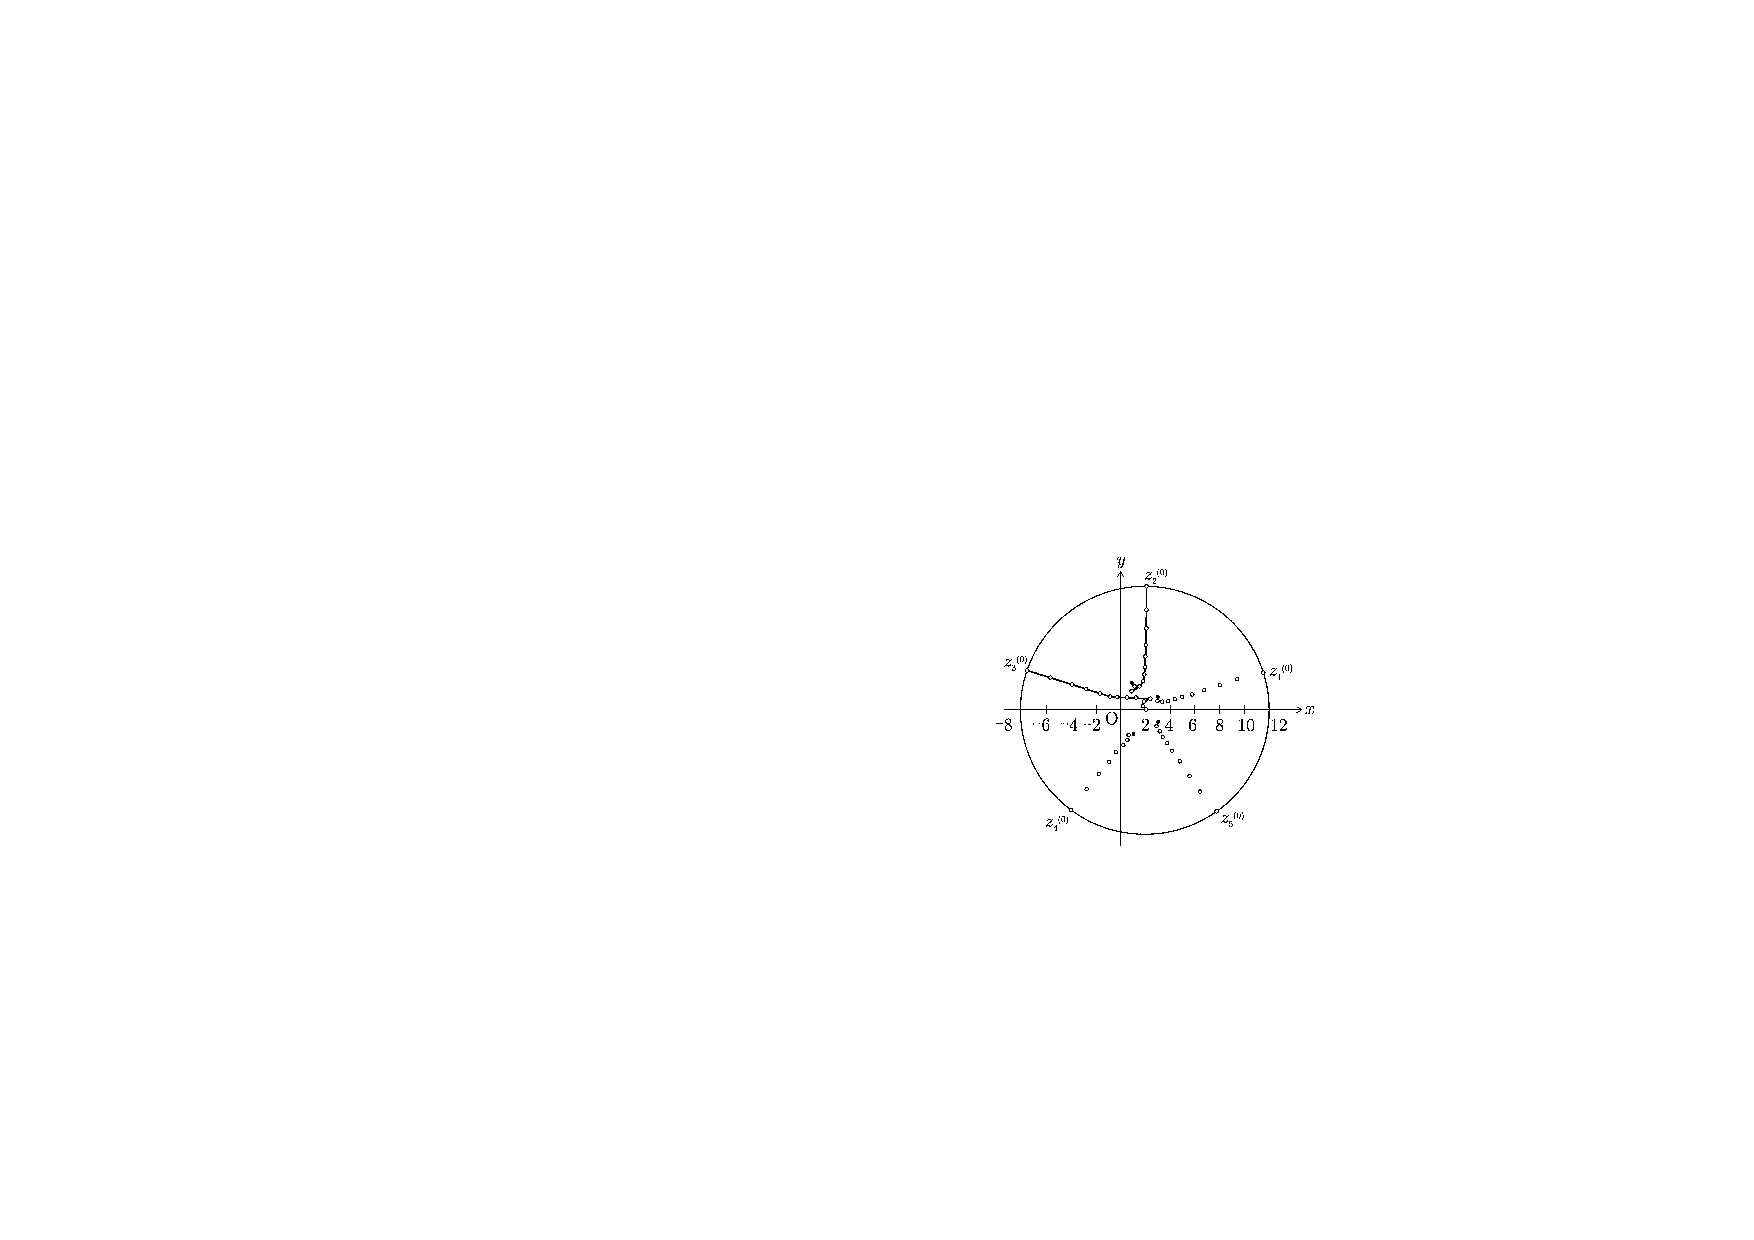
\includegraphics{image/DKA.pdf}}
\end{frame}

\section{行列演算}
% -*- coding: utf-8 -*-

\documentclass[10pt,dvipdfmx]{beamer}
\usepackage{tutorial}

\begin{document}
\section{行列とLAPACK}
\begin{frame}[t,fragile]{二次元配列}
  \begin{itemize}
    %\setlength{\itemsep}{1em}
  \item C言語では、二次元配列は一次元配列の先頭をさす(ポインタ)の配列として表される(と理解しておけば良い)
  \item \verb+a[i]+は、要素\verb+a[i][0]+を指すポインタ
    \begin{itemize}
    \item \verb+a+ と \verb+&a[0]+ は等価 (\verb+&a[0][0]+ ではない)
    \item \verb+a[0]+ と \verb+&a[0][0]+ は等価
    \item \verb+a[2]+ と \verb+&a[2][0]+ は等価
    \item \verb^(a+2)^ と \verb^&a[2]^ は等価
    \item \verb^(*(a+2))[3]^ と \verb^*(*(a+2)+3)^ と \verb^a[2][3]^ は等価
    \item \verb^*(a+2)[3]^ と \verb^*((a+2)[3])^ と \verb^*(a[5])^ と\verb^a[5][0]^ は等価
    \item \verb^[]^は\verb^*^よりも優先度が高い
    \end{itemize}
  \item ポインタのテストプログラム: \href{https://github.com/todo-group/computer-experiments/blob/master/exercise/matrix/pointer-matrix.c}{pointer-matrix.c}
  \end{itemize}
\end{frame}

\begin{frame}[t,fragile]{動的二次元配列の確保}
  \begin{itemize}
    \setlength{\itemsep}{1em}
  \item 各行を表す配列とそれぞれの先頭アドレスを保持する配列の二種類が必要
\begin{lstlisting}
double **a;
m = 10;  
n = 10;  
a = (double**)malloc((size_t)(m * sizeof(double*));
for (int i = 0; i < m; ++i)
  a[i] = (double*)malloc((size_t)(n * sizeof(double));
\end{lstlisting}
\item 各行を保持する配列が、メモリ上で連続に確保される保証はない
\item 行列用のライブラリ(LAPACK等)を使うときに問題となる
  \end{itemize}
\end{frame}

\begin{frame}[t,fragile]{BLASライブラリ}
  \begin{itemize}
    \setlength{\itemsep}{1em}
  \item 行列・行列積、行列・ベクトル積などを高速に行う最適化された関数群
  \item 行列・行列積を計算するサブルーチン {\tt dgemm} \\
    \url{http://www.netlib.org/lapack/explore-html/d7/d2b/dgemm_8f.html}
    \begin{itemize}
    \item $C = \alpha A \times B + \beta C$ を計算
    \item BLASもFortranで書かれている
    \end{itemize}
  \item 例: \href{https://github.com/todo-group/computer-experiments/blob/master/exercise/matrix/multiply.c}{multiply.c}, \href{https://github.com/todo-group/computer-experiments/blob/master/exercise/matrix/multiply_dgemm.c}{multiply\_dgemm.c}
  \end{itemize}
\end{frame}

\begin{frame}[t,fragile]{LAPACK (Linear Algebra PACKage)}
  \begin{itemize}
    %\setlength{\itemsep}{1em}
  \item 線形計算のための高品質な数値計算ライブラリ
    \begin{itemize}
    \item \url{http://www.netlib.org/lapack}
    \item 線形方程式、固有値問題、特異値問題、線形最小二乗問題など
    \item (FFT 高速フーリエ変換は入っていない)
    % \item LAPACK自体もFortran言語で書かれている
    \end{itemize}
  \item ほぼ全てのPC、ワークステーション、スーパーコンピュータで利用可 (インストール済)
  \item Netlibでソースが公開されているリファレンス実装は遅いが、それぞれのベンダー(Intel、Fujitsu、etc)による最適化されたLAPACKが用意されている場合が多い(MKL、SSL2、etc)
  \item LAPACKを使うことにより、高速で信頼性が高く、ポータブルなコードを書くことが可能になる
  \end{itemize}
\end{frame}

\begin{frame}[t,fragile]{LAPACKによる連立一次方程式の求解}
  \begin{itemize}
    \setlength{\itemsep}{1em}
  \item LU分解を行うサブルーチン {\tt dgetrf} \\
    \url{http://www.netlib.org/lapack/explore-html/d3/d6a/dgetrf_8f.html}
  \item Fortranによる関数宣言
\begin{lstlisting}
subroutine dgetrf(integer M, integer N,
         double precision, dimension(lda, *) A,
         integer LDA, integer, dimension(*) IPIV,
         integer INFO)
\end{lstlisting}
\item {\tt A}: 左辺の行列、{\tt M,N}: 次元、{\tt IPIV}: 選択されたピボット行のリスト、{\tt lda}: 通常{\tt M} (行数)と同じで良い
  \end{itemize}
\end{frame}

\begin{frame}[t,fragile]{CからBLAS/LAPACKを呼び出す際の注意事項}
  \begin{itemize}
    %\setlength{\itemsep}{1em}
  \item (もともとFortran言語で書かれていたことによる制限)
  \item 関数名はすべて小文字、最後に \verb+_+ (下線)を付ける
  \item スカラー、ベクトル、行列は全て「ポインタ渡し」とする
  \item ベクトルや行列は最初の要素へのポインタを渡す (サイズは別に渡す)
  \item 行列の要素は(0,0) $\rightarrow$ (1,0) $\rightarrow$ (2,0) $\rightarrow\cdots\rightarrow$ $(m-1,0)$ $\rightarrow$ (0,1) $\rightarrow$ (1,1) $\rightarrow\cdots\rightarrow$ $(m-1,n-1)$の順で連続して並んでいなければならない(column-major)
    \begin{itemize}
    \item C言語の二次元配列では \verb+a[i][j]+ の次には \verb%a[i][j+1]%が入っている(row-major)
    \item 行列が転置されて解釈されてしまう!
    \end{itemize}
  \item コンパイル時には{\tt -llapack -lblas}オプションを指定し、LAPACKライブラリとBLASライブラリをリンクする(ハンドブック2.1.6節)
  \end{itemize}
\end{frame}

\begin{frame}[t,fragile]{cmatrix.hライブラリ}
  \begin{itemize}
    %\setlength{\itemsep}{1em}
  \item Column-major形式の二次元配列の確保({\tt alloc\_dmatrix})、開放({\tt free\_dmatrix})、出力({\tt print\_dmatrix})、読み込み({\tt read\_dmatrix})を行うためのユーティリティ関数、(i,j)成分にアクセスするためのマクロ({\tt mat\_elem})他を準備
  \item ソースコード: \href{https://github.com/todo-group/computer-experiments/blob/master/exercise/matrix/cmatrix.h}{cmatrix.h}
  \item 使用例
\begin{lstlisting}
#include "cmatrix.h"
...
double **mat;
mat = alloc_dmatrix(m, n);
mat_elem(mat, 1, 3) = 5.0;
...
free_dmatrix(mat);
\end{lstlisting}
  \item サンプルコード: \href{https://github.com/todo-group/computer-experiments/blob/master/exercise/matrix/matrix_example.c}{matrix\_example.c}
  \end{itemize}
\end{frame}

\begin{frame}[t,fragile]{alloc\_dmatrixでの動的二次元配列の確保}
  \begin{itemize}
    %\setlength{\itemsep}{1em}
  \item 長さ$m \times n$の一次元配列を用意し、各列(それぞれ$m$要素)の先頭アドレスを長さ$n$のポインター配列に格納する (ハンドブック2.12.3節)
\begin{lstlisting}
double **a;
m = 10;  
n = 10;  
a = (double**)malloc((size_t)(n * sizeof(double*));
a[0] = (double*)malloc((size_t)(m*n * sizeof(double));
for (int i = 1; i < n; ++i)
  a[i] = a[i-1] + m;
\end{lstlisting}
\item 行列の(i,j)成分を\verb+a[j][i]+に格納することにする (column-major)
  \end{itemize}
\end{frame}

\begin{frame}[t,fragile]{要素アクセス・先頭アドレス}
  \begin{itemize}
    % \setlength{\itemsep}{1em}
  \item 行列の(i,j)成分は\verb+a[j][i]+に格納されている
    \begin{itemize}
      \item \href{https://github.com/todo-group/computer-experiments/blob/master/exercise/matrix/cmatrix.h}{cmatrix.h}ではマクロ(\verb+mat_elem+)を準備
\begin{lstlisting}
#define mat_elem(mat, i, j) (mat)[j][i]
\end{lstlisting}
\item このマクロを使うと、例えば(i,j)成分への代入は以下のように書ける
\begin{lstlisting}
mat_elem(a, i, j) = 1;
\end{lstlisting}
\end{itemize}
  \item LAPACKにベクトルや行列の最初の要素へのポインタを渡す
    \begin{itemize}
      \item ベクトルの最初の要素(0)へのポインタ: \verb+&v[0]+
      \item 行列の最初の要素(0,0)へのポインタ: \verb+&a[0][0]+
      \item \href{https://github.com/todo-group/computer-experiments/blob/master/exercise/matrix/cmatrix.h}{cmatrix.h}にマクロ({\tt vec\_ptr}、{\tt mat\_ptr})が準備されているのでそれぞれ、{\tt vec\_ptr(v)}、{\tt mat\_ptr(a)}と書ける
    \end{itemize}
  \end{itemize}
\end{frame}

\begin{frame}[t,fragile]{LAPACKによる連立一次方程式の求解}
  \begin{itemize}
    \setlength{\itemsep}{1em}
  \item C言語から呼び出すための関数宣言を作成 (ハンドブック2.7.4節)
\begin{lstlisting}
void dgetrf_(int *M, int *N, double *A,
             int *LDA, int*IPIV, int *INFO);
\end{lstlisting}
関数名は全て小文字。関数名の最後に {\tt \_} (下線)を付ける
\item LU分解の例
\begin{lstlisting}
m = 10;
n = 10;
a = alloc_dmatrix(m, n);
...
dgetrf_(&m, &n, mat_ptr(a), &m, vec_ptr(ipiv), &info);
\end{lstlisting}
完全なソースコード: \href{https://github.com/todo-group/computer-experiments/blob/master/exercise/linear_system/lu_decomp.c}{lu\_decomp.c}
  \end{itemize}
\end{frame}

\end{document}

\section{複素数}
\begin{frame}[t,fragile]{複素数}
  \begin{itemize}
    %\setlength{\itemsep}{1em}
  \item {\tt complex.h}をincludeすることで、double complex 型 (float complex 型)が使えるようになる
  \item 複素数の値は、{\tt CMPLX} (あるいは{\tt CMPLXF})で設定する
  \item {\tt cexp}, {\tt csin}, {\tt clog}等の初等関数が使える
  \item 実部は{\tt creal}, 虚部は{\tt cimag}で取り出せる
  \item プログラム例: \href{https://github.com/todo-group/computer-experiments/blob/master/exercise/basics/complex.c}{complex.c}
\begin{lstlisting}
#include <complex.h>
...
double complex x, y;
x = CMPLX(0, 1); /* 虚数単位 */
y = cexp(x * M_PI);
printf("i = (%lf,%lf)\n", creal(x), cimag(x));
printf("e^{i*pi} = (%lf,%lf)\n", creal(y), cimag(y));
\end{lstlisting}
  \end{itemize}
\end{frame}

% -*- coding: utf-8 -*-

\section{C言語における行列・LAPACKの利用}

\begin{frame}[t,fragile]{C言語におけるポインタ}
  \begin{itemize}
    \setlength{\itemsep}{1em}
  \item 変数はメモリ上のどこかに格納されている
    \begin{itemize}
    \item 変数の値: メモリに格納されている数値
    \item アドレス: 変数の値が格納されているメモリ上の番地
    \end{itemize}
  \item ポインタ変数
    \begin{itemize}
    \item 値としてアドレスを格納する変数のこと
    \item ポインタ変数の値(アドレス)とポインタ変数のアドレスは異なるものであることに注意
    \end{itemize}
  \item ポインタ変数の宣言、代入、実体へのアクセス
    \begin{itemize}
    \item 整数型ポインタ変数の宣言: {\color{red} \verb+int *p;+}
    \item 整数型変数の宣言: \verb+int q;+
    \item 変数\verb+q+のアドレスをポインタ変数\verb+p+に代入: {\color{red} \verb+p = &q;+}
    \item ポインタ変数\verb+p+に格納されているアドレスに格納されている値の参照(間接参照): {\color{red} \verb+*p+}
    \end{itemize}
  \end{itemize}
\end{frame}

\begin{frame}[t,fragile]{ポインタの例(1)}
  \begin{itemize}
    %\setlength{\itemsep}{1em}
  \item 例2.5.1 (ハンドブック2.5節)
\begin{lstlisting}
#include <stdio.h>
int main() {
  int *p;
  int q;
  q = 200;
  p = &q;
  printf("q is %d and *p is %d.\n", q, *p);
  return 0;
}
\end{lstlisting}
\begin{itemize}
\item \verb+q+のアドレスを\verb+p+に代入
\item \verb+q+と\verb+*p+の値を出力 → 両者とも200
\end{itemize}
  \end{itemize}
\end{frame}

\begin{frame}[t,fragile]{ポインタの例(2)}
  \begin{itemize}
    %\setlength{\itemsep}{1em}
  \item 例2.5.2 (ハンドブック2.5節)
\begin{lstlisting}
#include <stdio.h>
int main() {
  int *p;
  int q;
  p = &q;
  *p = 300;
  printf("q is %d and *p is %d.\n", q, *p);
  return 0;
}
\end{lstlisting}
\begin{itemize}
\item \verb+q+のアドレスを\verb+p+に代入
\item \verb+*p+に300を代入 (ここで\verb+q=300;+と書いても等価)
\item \verb+q+と\verb+*p+の値を出力 → 両者とも300
\end{itemize}
  \end{itemize}
\end{frame}

\begin{frame}[t,fragile]{関数呼び出し(ポインタ渡し)}
  \begin{itemize}
    %\setlength{\itemsep}{1em}
  \item 例2.7.4 (ハンドブック2.7節)
\begin{lstlisting}
#include <stdio.h>
void division(int divident, int divisor, int *quotient,
              int *residual) {
  *quotient = divident / divisor;
  *residual = divident % divisor;
}
int main() {
  int josuu = 3;
  int hi_josuu = 13;
  int shou, amari;
  division(hi_josuu, josuu, &shou, &amari);
  printf("%d / %d = %d ... %d\n", hi_josuu, josuu,
         shou, amari);
}
\end{lstlisting}
  \end{itemize}
\end{frame}

\begin{frame}[t,fragile]{間違った例(値渡し)}
  \begin{itemize}
    %\setlength{\itemsep}{1em}
  \item 例2.7.5 (ハンドブック2.7節)
\begin{lstlisting}
#include <stdio.h>
void division(int divident, int divisor, int quotient,
  int residual) {
  quotient = divident / divisor;
  residual = divident % divisor;
}
int main() {
  int josuu = 3;
  int hi_josuu = 13;
  int shou, amari;
  division(hi_josuu, josuu, shou, amari);
  printf("%d / %d = %d ... %d\n", hi_josuu, josuu,
         shou, amari);
}
\end{lstlisting}
\begin{itemize}
\item 誤った答えが出力される。なぜ?
\end{itemize}
  \end{itemize}
\end{frame}

\begin{frame}[t,fragile]{一次元配列}
  \begin{itemize}
    \setlength{\itemsep}{1em}
  \item (静的)一次元配列 (ハンドブック3.3.1節)
\begin{lstlisting}
double v[10];
v[0] = 1.0;
v[1] = 2.0;
...
\end{lstlisting}
    要素数はコンパイル時にすでに決まっている定数でなければならない
  \item (動的)一次元配列 (ハンドブック3.11節)
\begin{lstlisting}
double *v; /* ポインタ */
v = (double*)malloc((size_t)(10 * sizeof(double));
...
free(v); /* 確保した領域を開放 */
\end{lstlisting}
実行時に要素数を指定可能
  \end{itemize}
\end{frame}

\begin{frame}[t,fragile]{ポインタと一次元配列}
  \begin{itemize}
    %\setlength{\itemsep}{1em}
  \item 一次元配列を表す変数は、(実は)最初の要素を指すポインタ  (ハンドブック2.5.3節)
    \begin{itemize}
    \item \verb+v+ と \verb+&v[0]+ は等価
    \item \verb^(v+2)^ と \verb^&v[2]^ は等価
    \item \verb+*v+ と \verb+v[0]+ は等価
    \item \verb^*(v+2)^ と \verb^v[2]^ は等価
    \item \verb^(v+2)[3]^ は?
    \end{itemize}
  \item C言語では配列の添字は0から始まることに注意
  \item \verb^double v[10];^ と宣言した場合、\verb^v[0]^ 〜 \verb^v[9]^ の10個の要素を持つ配列が作られる。\verb^v[10]^ は存在しない。値を代入したり参照しようとするとエラーとなる
  \item ポインタのテストプログラム: \href{https://github.com/todo-group/computer-experiments/blob/master/exercise/matrix/pointer.c}{pointer.c}
  \end{itemize}
\end{frame}

\begin{frame}[t,fragile]{二次元配列}
  \begin{itemize}
    %\setlength{\itemsep}{1em}
  \item C言語では、二次元配列は一次元配列の先頭をさす(ポインタ)の配列として表される(と理解しておけば良い)
  \item \verb+a[i]+は、要素\verb+a[i][0]+を指すポインタ
    \begin{itemize}
    \item \verb+a+ と \verb+&a[0]+ は等価 (\verb+&a[0][0]+ ではない)
    \item \verb+a[0]+ と \verb+&a[0][0]+ は等価
    \item \verb+a[2]+ と \verb+&a[2][0]+ は等価
    \item \verb^(a+2)^ と \verb^&a[2]^ は等価
    \item \verb^(*(a+2))[3]^ と \verb^*(*(a+2)+3)^ と \verb^a[2][3]^ は等価
    \item \verb^*(a+2)[3]^ と \verb^*((a+2)[3])^ と \verb^*(a[5])^ と\verb^a[5][0]^ は等価
    \item \verb^[]^は\verb^*^よりも優先度が高い
    \end{itemize}
  \item ポインタのテストプログラム: \href{https://github.com/todo-group/computer-experiments/blob/master/exercise/matrix/pointer-matrix.c}{pointer-matrix.c}
  \end{itemize}
\end{frame}

\begin{frame}[t,fragile]{動的二次元配列の確保}
  \begin{itemize}
    \setlength{\itemsep}{1em}
  \item 各行を表す配列とそれぞれの先頭アドレスを保持する配列の二種類が必要
\begin{lstlisting}
double **a;
m = 10;  
n = 10;  
a = (double**)malloc((size_t)(m * sizeof(double*));
for (int i = 0; i < m; ++i)
  a[i] = (double*)malloc((size_t)(n * sizeof(double));
\end{lstlisting}
\item 各行を保持する配列が、メモリ上で連続に確保される保証はない
\item 行列用のライブラリ(LAPACK等)を使うときに問題となる
  \end{itemize}
\end{frame}

\begin{frame}[t,fragile]{BLASライブラリ}
  \begin{itemize}
    \setlength{\itemsep}{1em}
  \item 行列・行列積、行列・ベクトル積などを高速に行う最適化された関数群
  \item 行列・行列積を計算するサブルーチン {\tt dgemm} \\
    \url{http://www.netlib.org/lapack/explore-html/d7/d2b/dgemm_8f.html}
    \begin{itemize}
    \item $C = \alpha A \times B + \beta C$ を計算
    \item BLASもFortranで書かれている
    \end{itemize}
  \item 例: \href{https://github.com/todo-group/computer-experiments/blob/master/exercise/matrix/multiply.c}{multiply.c}, \href{https://github.com/todo-group/computer-experiments/blob/master/exercise/matrix/multiply_dgemm.c}{multiply\_dgemm.c}
  \end{itemize}
\end{frame}

\begin{frame}[t,fragile]{LAPACK (Linear Algebra PACKage)}
  \begin{itemize}
    %\setlength{\itemsep}{1em}
  \item 線形計算のための高品質な数値計算ライブラリ
    \begin{itemize}
    \item \url{http://www.netlib.org/lapack}
    \item 線形方程式、固有値問題、特異値問題、線形最小二乗問題など
    \item (FFT 高速フーリエ変換は入っていない)
    % \item LAPACK自体もFortran言語で書かれている
    \end{itemize}
  \item ほぼ全てのPC、ワークステーション、スーパーコンピュータで利用可 (インストール済)
  \item Netlibでソースが公開されているリファレンス実装は遅いが、それぞれのベンダー(Intel、Fujitsu、etc)による最適化されたLAPACKが用意されている場合が多い(MKL、SSL2、etc)
  \item LAPACKを使うことにより、高速で信頼性が高く、ポータブルなコードを書くことが可能になる
  \end{itemize}
\end{frame}

\begin{frame}[t,fragile]{LAPACKによる連立一次方程式の求解}
  \begin{itemize}
    \setlength{\itemsep}{1em}
  \item LU分解を行うサブルーチン {\tt dgetrf} \\
    \url{http://www.netlib.org/lapack/explore-html/d3/d6a/dgetrf_8f.html}
  \item Fortranによる関数宣言
\begin{lstlisting}
subroutine dgetrf(integer M, integer N,
         double precision, dimension(lda, *) A,
         integer LDA, integer, dimension(*) IPIV,
         integer INFO)
\end{lstlisting}
\item {\tt A}: 左辺の行列、{\tt M,N}: 次元、{\tt IPIV}: 選択されたピボット行のリスト、{\tt lda}: 通常{\tt M} (行数)と同じで良い
  \end{itemize}
\end{frame}

\begin{frame}[t,fragile]{CからBLAS/LAPACKを呼び出す際の注意事項}
  \begin{itemize}
    %\setlength{\itemsep}{1em}
  \item (もともとFortran言語で書かれていたことによる制限)
  \item 関数名はすべて小文字、最後に \verb+_+ (下線)を付ける
  \item スカラー、ベクトル、行列は全て「ポインタ渡し」とする
  \item ベクトルや行列は最初の要素へのポインタを渡す (サイズは別に渡す)
  \item 行列の要素は(0,0) $\rightarrow$ (1,0) $\rightarrow$ (2,0) $\rightarrow\cdots\rightarrow$ $(m-1,0)$ $\rightarrow$ (0,1) $\rightarrow$ (1,1) $\rightarrow\cdots\rightarrow$ $(m-1,n-1)$の順で連続して並んでいなければならない(column-major)
    \begin{itemize}
    \item C言語の二次元配列では \verb+a[i][j]+ の次には \verb%a[i][j+1]%が入っている(row-major)
    \item 行列が転置されて解釈されてしまう!
    \end{itemize}
  \item コンパイル時には{\tt -llapack -lblas}オプションを指定し、LAPACKライブラリとBLASライブラリをリンクする(ハンドブック2.1.6節)
  \end{itemize}
\end{frame}

\begin{frame}[t,fragile]{cmatrix.hライブラリ}
  \begin{itemize}
    %\setlength{\itemsep}{1em}
  \item Column-major形式の二次元配列の確保({\tt alloc\_dmatrix})、開放({\tt free\_dmatrix})、出力({\tt print\_dmatrix})、読み込み({\tt read\_dmatrix})を行うためのユーティリティ関数、(i,j)成分にアクセスするためのマクロ({\tt mat\_elem})他を準備
  \item ソースコード: \href{https://github.com/todo-group/computer-experiments/blob/master/exercise/matrix/cmatrix.h}{cmatrix.h}
  \item 使用例
\begin{lstlisting}
#include "cmatrix.h"
...
double **mat;
mat = alloc_dmatrix(m, n);
mat_elem(mat, 1, 3) = 5.0;
...
free_dmatrix(mat);
\end{lstlisting}
  \item サンプルコード: \href{https://github.com/todo-group/computer-experiments/blob/master/exercise/matrix/matrix_example.c}{matrix\_example.c}
  \end{itemize}
\end{frame}

\begin{frame}[t,fragile]{alloc\_dmatrixでの動的二次元配列の確保}
  \begin{itemize}
    %\setlength{\itemsep}{1em}
  \item 長さ$m \times n$の一次元配列を用意し、各列(それぞれ$m$要素)の先頭アドレスを長さ$n$のポインター配列に格納する (ハンドブック2.12.3節)
\begin{lstlisting}
double **a;
m = 10;  
n = 10;  
a = (double**)malloc((size_t)(n * sizeof(double*));
a[0] = (double*)malloc((size_t)(m*n * sizeof(double));
for (int i = 1; i < n; ++i)
  a[i] = a[i-1] + m;
\end{lstlisting}
\item 行列の(i,j)成分を\verb+a[j][i]+に格納することにする (column-major)
  \end{itemize}
\end{frame}

\begin{frame}[t,fragile]{要素アクセス・先頭アドレス}
  \begin{itemize}
    % \setlength{\itemsep}{1em}
  \item 行列の(i,j)成分は\verb+a[j][i]+に格納されている
    \begin{itemize}
      \item \href{https://github.com/todo-group/computer-experiments/blob/master/exercise/matrix/cmatrix.h}{cmatrix.h}ではマクロ(\verb+mat_elem+)を準備
\begin{lstlisting}
#define mat_elem(mat, i, j) (mat)[j][i]
\end{lstlisting}
\item このマクロを使うと、例えば(i,j)成分への代入は以下のように書ける
\begin{lstlisting}
mat_elem(a, i, j) = 1;
\end{lstlisting}
\end{itemize}
  \item LAPACKにベクトルや行列の最初の要素へのポインタを渡す
    \begin{itemize}
      \item ベクトルの最初の要素(0)へのポインタ: \verb+&v[0]+
      \item 行列の最初の要素(0,0)へのポインタ: \verb+&a[0][0]+
      \item \href{https://github.com/todo-group/computer-experiments/blob/master/exercise/matrix/cmatrix.h}{cmatrix.h}にマクロ({\tt vec\_ptr}、{\tt mat\_ptr})が準備されているのでそれぞれ、{\tt vec\_ptr(v)}、{\tt mat\_ptr(a)}と書ける
    \end{itemize}
  \end{itemize}
\end{frame}

\begin{frame}[t,fragile]{LAPACKによる連立一次方程式の求解}
  \begin{itemize}
    \setlength{\itemsep}{1em}
  \item C言語から呼び出すための関数宣言を作成 (ハンドブック2.7.4節)
\begin{lstlisting}
void dgetrf_(int *M, int *N, double *A,
             int *LDA, int*IPIV, int *INFO);
\end{lstlisting}
関数名は全て小文字。関数名の最後に {\tt \_} (下線)を付ける
\item LU分解の例
\begin{lstlisting}
m = 10;
n = 10;
a = alloc_dmatrix(m, n);
...
dgetrf_(&m, &n, mat_ptr(a), &m, vec_ptr(ipiv), &info);
\end{lstlisting}
完全なソースコード: \href{https://github.com/todo-group/computer-experiments/blob/master/exercise/linear_system/lu_decomp.c}{lu\_decomp.c}
  \end{itemize}
\end{frame}


% -*- coding: utf-8 -*-

\section{二分法}

\begin{frame}[t,fragile]{二分法}
  \begin{itemize}
    % \setlength{\itemsep}{1em}
  \item 反復法により一次元の方程式$f(x)=0$の解を求める
  \item 導関数を使わず関数値のみを利用 (c.f. ニュートン法)
  \item 初期条件として、$f(a) \times f(b) < 0$を満たす2点の組($a<b$)で解をはさみ込み、領域を狭めていく
  \item $a$と$b$の中点$x=(a+b)/2$を考える
    \begin{itemize}
    \item $|f(x)|$が十分小さい場合: $x$が解
    \item $f(a) \times f(x) < 0$の場合: $[a,x]$を新しい領域にとる
    \item $f(x) \times f(b) < 0$の場合: $[x,b]$を新しい領域にとる
    \end{itemize}
  \item 領域$[a,b]$の幅が十分小さくなったら終了
  \item 反復のたびに領域の幅は半分になる
  \item 全ての解を得られる保証はない
  \item 二分法の例: \href{https://github.com/todo-group/computer-experiments/blob/master/exercise/basics/bisection.c}{bisection.c}
  \end{itemize}
\end{frame}


\section{実習その3}

\begin{frame}[t,fragile]{EX3-1: サンプルプログラムの実行}
  \begin{itemize}
    %\setlength{\itemsep}{1em}
  \item[3-1-1] ガウスの消去法のサンプルプログラム(\href{https://github.com/todo-group/computer-experiments/blob/master/exercise/linear_system/gauss.c}{exercise/linear\_system/gauss.c})をコンパイル・実行せよ。実行時にコマンドライン引数に行列の内容が書かれたファイル名({\tt input1.dat})を指定する必要があることに注意
\begin{lstlisting}
$ cc gauss.c -o gauss
$ ./gauss input1.dat
\end{lstlisting}
  \item[3-1-2] LU分解のサンプルプログラム(\href{https://github.com/todo-group/computer-experiments/blob/master/exercise/linear_system/lu_decomp.c}{exercise/linear\_system/lu\_decomp.c})をコンパイル・実行せよ。コンパイル時にLAPACKをリンク({\tt -llapack})する必要があることに注意(ハンドブック3.1.6節)
\begin{lstlisting}
$ cc lu_decomp.c -o lu_decomp -llapack
$ ./lu_decomp input1.dat
\end{lstlisting}
  \end{itemize}
\end{frame}

\begin{frame}[t,fragile]{EX3-2: ピボット選択、境界条件}
  \begin{itemize}
    %\setlength{\itemsep}{1em}
  \item[3-2-1] {\tt gauss.c}では、ピボット選択を行っていないため、入力が{\tt input2.dat}の場合には正しい解が得られない。ピボット選択を行うよう{\tt gauss.c}を修正せよ
  \item[3-2-2] \href{https://github.com/todo-group/computer-experiments/blob/master/exercise/linear_system/laplace_lu.c}{exercise/linear\_system/laplace\_lu.c}では、ディリクレ型の境界条件[$u(0,y) = \sin(\pi y)$, $u(x,0)=u(x,1)=u(1,y)=0$]のもとでのラプラス方程式の解をLU分解により求めている。境界条件を変えてみて解がどのように変化するか、Gnuplotを用いてプロットして確認せよ(Gnuplotの{\tt splot}コマンドを使う)
  \end{itemize}
\end{frame}

\begin{frame}[t,fragile]{EX3-3: ヤコビ法、ガウス・ザイデル法、SOR法}
  \begin{itemize}
    %\setlength{\itemsep}{1em}
  \item[3-3-1] \href{https://github.com/todo-group/computer-experiments/exercise/blob/master/linear_system/laplace_jacobi.c}{exercise/linear\_system/laplace\_jacobi.c}は、作りかけのヤコビ法のプログラムである。収束判定のコードを追加し、プログラムを完成せよ。計算結果や計算速度を{\tt laplace\_lu.c}と比較せよ
  \item[3-3-2] ヤコビ法のプログラム({\tt lapalace\_jacobi.c})を元に、ガウス・ザイデル法、SOR法のプログラムを作成せよ。収束までの回数を比較せよ。
特にSOR法の場合、パラメータ$\omega$の選び方により、どのように収束回数が変化するか観察し、最適な$\omega$の値について考察せよ
  \end{itemize}
\end{frame}


\end{document}
